% Section VII: Empirical Results. Scope-B rewrite: priority-respecting compromise
% (Figs 10/11/12), Theorem-4.1 in deployment (Fig 18), wall-time benefit (Fig 22),
% qualitative C1-vs-C4 overlay (Fig 28), §8.5 diagnostics table, §10 necessity table.

This section reports the empirical evidence supporting the deployment claim of Section~\ref{sec:intro:contributions}: that the calibrated weighted-sum planner produces priority-respecting compromise on every scenario in the benchmark, reproduces the formal lex cascade's per-tick compliance pattern at the top priority levels, and runs at a small fraction of the cascade's wall-time. The evidence is organised against the four empirical objects of Section~\ref{sec:protocol:objects}: per-level integrated violation (\S\ref{sec:results:compromise}), per-tick compliance match $C_1$-vs-$C_4$ (\S\ref{sec:results:theorem41}), per-scenario wall time (\S\ref{sec:results:cost}), and the framework-side scans (\S\ref{sec:results:framework}).

\subsection{Priority-Respecting Compromise}
\label{sec:results:compromise}

\begin{figure}[t]
    \centering
    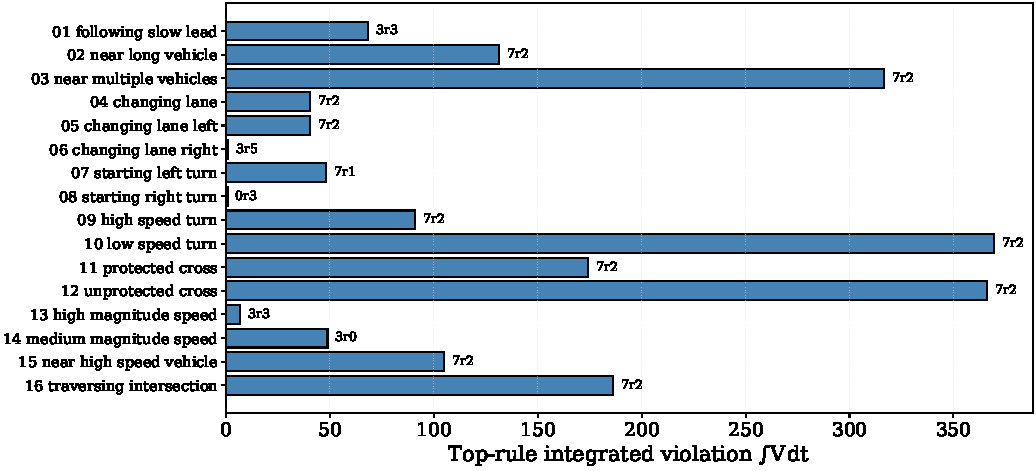
\includegraphics[width=\linewidth]{./Figures/fig10_top_violation}
    \caption{Per-scenario top-rule integrated violation under the operational LCP planner $C_1$, restricted to the 13 MPC-controlled rules of Section~\ref{sec:rulebook:partition} (Definition~\ref{def:per-level-violation}). Bar length is $\int V \, dt$ over the scenario's worst-violating MPC-controlled rule; the bar annotation gives the rule ID. Across the 16 scenarios the top-violating MPC rule lives at $L_0$ on 1 scenario, $L_3$ on 4 scenarios, and $L_7$ on 11 scenarios; the rule IDs encountered are $\texttt{0r3}$, $\texttt{3r0}$, $\texttt{3r3}$, $\texttt{3r5}$, $\texttt{7r1}$, $\texttt{7r2}$. Collision-avoidance levels $L_8$, $L_9$, $L_{10}$ never appear as the top-violating MPC rule: the planner holds them effectively hard on every scenario.}
    \label{fig:top_violation}
\end{figure}

\begin{figure}[t]
    \centering
    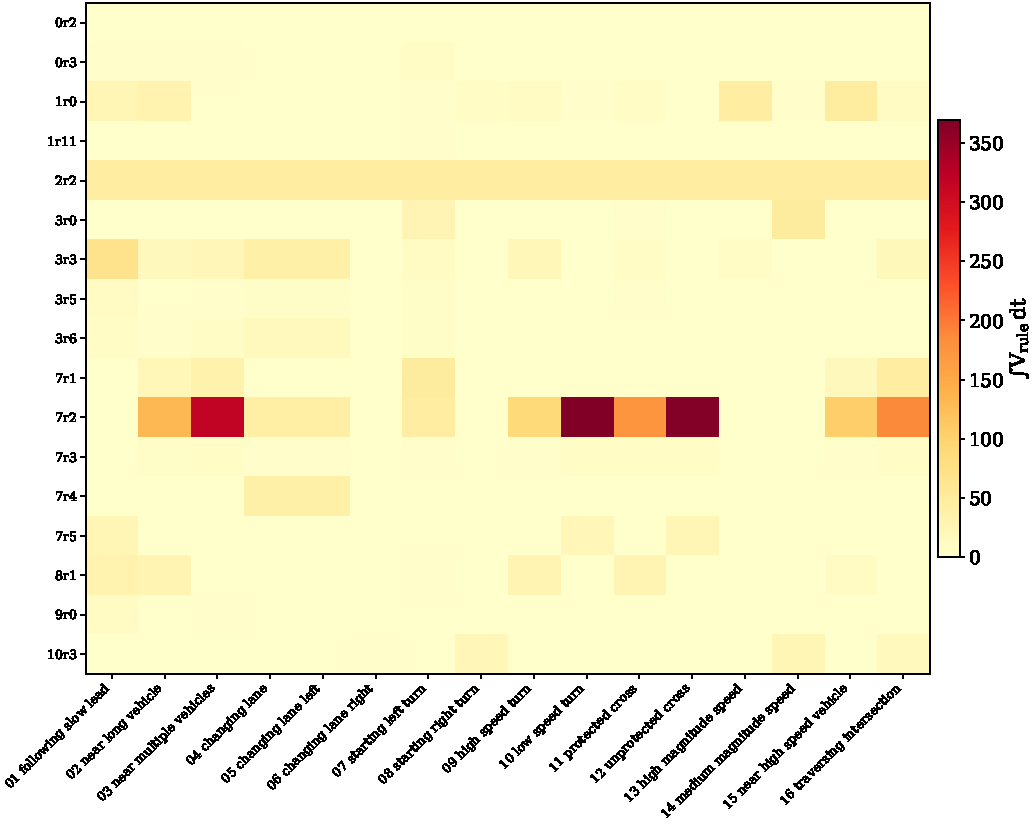
\includegraphics[width=\linewidth]{./Figures/fig11_rule_scenario_heatmap}
    \caption{Per-rule per-scenario integrated-violation heatmap under $C_1$. Rows are rule IDs sorted by descending priority level; columns are scenarios. Cell intensity is $\int V_{\mathrm{rule}} \, dt$. The heatmap visualises the priority structure of the compromise: the top rows (high-priority rules) are uniformly cold across scenarios, the bottom rows (low-priority comfort and speed rules) carry the bulk of the violation mass.}
    \label{fig:rule_scenario_heatmap}
\end{figure}

\begin{figure}[t]
    \centering
    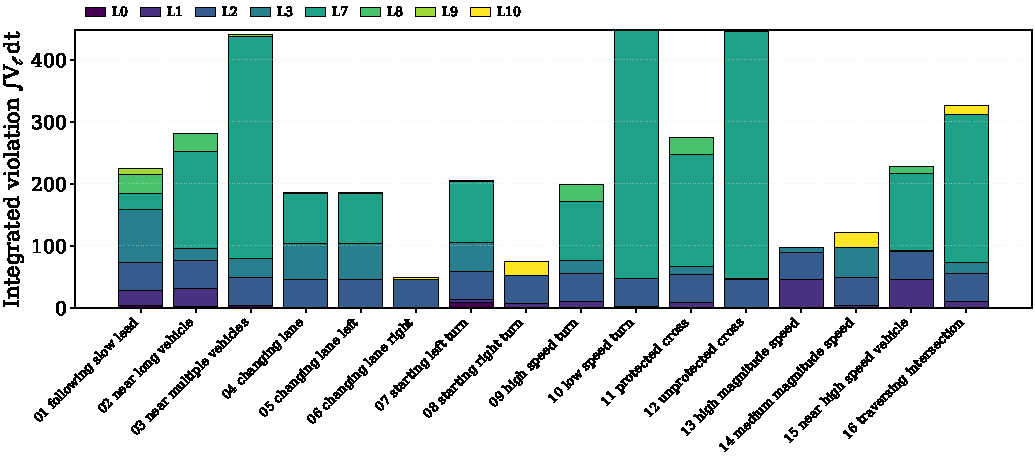
\includegraphics[width=\linewidth]{./Figures/fig12_level_breakdown}
    \caption{Per-scenario stacked breakdown of $V_\ell^{(C_1, s)}$ by priority level (Definition~\ref{def:per-level-violation}). Each bar's segments correspond to priority levels (lighter shade = lower priority). The stacking pattern is invariant across scenarios: low-priority levels accumulate visibly while high-priority levels remain a thin band at the top.}
    \label{fig:level_breakdown}
\end{figure}

Figures~\ref{fig:top_violation}--\ref{fig:level_breakdown} address the central deployment claim. Three complementary views of the same per-tick observer data establish the same pattern: the operational LCP planner $C_1$ concentrates MPC-controlled rule violations at the legal and comfort levels ($L_7$, $L_3$, $L_0$) and holds the collision-avoidance levels ($L_8$, $L_9$, $L_{10}$) effectively hard on every scenario. Figure~\ref{fig:top_violation} shows that the worst-violating MPC rule per scenario lives at $L_7$ (11 of 16 scenarios; the geometrically forced opposing-lane and traffic-light constraints during turns), $L_3$ (4 of 16; speed-limit and safe-headway compromises during dense-traffic following), or $L_0$ (1 of 16; lateral-comfort compromise during a sharp right turn). Figure~\ref{fig:rule_scenario_heatmap} disaggregates by rule and scenario; the high-priority rule rows (the four MPC-controlled rules at $L_8$--$L_{10}$) are uniformly cold across scenarios, while the legal-and-below rule rows accumulate the visible violation mass. Figure~\ref{fig:level_breakdown} stacks per-level integrated violation per scenario; the stacking ordering --- collision-levels at the bottom holding near zero, legal-and-below levels carrying the violation mass --- is the same across all 16 scenarios. The shape of the priority-respecting compromise is therefore not scenario-specific --- it is a structural property of the planner.

Table~\ref{tab:per_scenario_status} summarises the per-scenario outcome: tick count, count of MPC-controlled rules with non-zero integrated violation, and the worst-violating MPC-controlled rule with its integrated value. The pattern is concentrated: across the 16 scenarios, the top-violating MPC rule is \texttt{7r2} (Opposing Lane, $L_7$) on 9 scenarios --- a geometrically forced relaxation during protected-cross, opposing-lane, and turning manoeuvres documented in Table~\ref{tab:necessity}; \texttt{7r1} (Traffic-Light Compliance, $L_7$) on \texttt{07\_starting\_left\_turn} --- geometrically forced during the sharp left turn at the signalised intersection; \texttt{3r3} (Safe Headway, $L_3$) on \texttt{01\_following\_slow\_lead} and \texttt{13\_high\_magnitude\_speed} --- the canonical comfort-tier compromise; \texttt{3r0} (Speed Limit, $L_3$) on \texttt{14\_medium\_magnitude\_speed}; \texttt{3r5} (Lateral Clearance, $L_3$) on \texttt{06\_changing\_lane\_right}; and \texttt{0r3} (Lateral Comfort, $L_0$) on \texttt{08\_starting\_right\_turn}. The two collision-avoidance MPC rules \texttt{10r0} (VRU) and \texttt{9r0} (non-VRU) never appear as the top-violating rule on any scenario and have zero integrated violation throughout the benchmark; observer-only level $L_8$ (mandatory-stop approach: \texttt{8r0}, \texttt{8r1}) has no MPC representative and is excluded from this comparison by construction. The pattern is the empirical signature of the planner holding the collision-avoidance levels effectively hard.

\begin{table}[t]
    \centering
    \caption{Per-scenario status under the operational LCP planner $C_1$ on the 16-scenario \texttt{nuPlan-mini} benchmark. The top-rule column is filtered to the 13 MPC-controlled rules of \S\ref{sec:rulebook:partition}; observer-only and stub rules are excluded since they are not under planner control.}
    \label{tab:per_scenario_status}
    \footnotesize
\begin{tabular}{lrrl}
\toprule
Scenario & Ticks & $\#$ viol.\ MPC rules & Top MPC rule (integrated) \\
\midrule
01\_following\_slow\_lead & 150 & 6 & \texttt{3r3} (68.44) \\
02\_near\_long\_vehicle & 150 & 8 & \texttt{7r2} (131.28) \\
03\_near\_multiple\_vehicles & 150 & 8 & \texttt{7r2} (316.43) \\
04\_changing\_lane & 149 & 6 & \texttt{7r2} (40.54) \\
05\_changing\_lane\_left & 149 & 6 & \texttt{7r2} (40.54) \\
06\_changing\_lane\_right & 150 & 3 & \texttt{3r5} (0.82) \\
07\_starting\_left\_turn & 150 & 10 & \texttt{7r1} (48.00) \\
08\_starting\_right\_turn & 150 & 3 & \texttt{0r3} (0.71) \\
09\_high\_speed\_turn & 149 & 5 & \texttt{7r2} (90.78) \\
10\_low\_speed\_turn & 149 & 6 & \texttt{7r2} (369.64) \\
11\_protected\_cross & 149 & 7 & \texttt{7r2} (174.15) \\
12\_unprotected\_cross & 149 & 6 & \texttt{7r2} (365.98) \\
13\_high\_magnitude\_speed & 149 & 2 & \texttt{3r3} (6.60) \\
14\_medium\_magnitude\_speed & 150 & 3 & \texttt{3r0} (48.81) \\
15\_near\_high\_speed\_vehicle & 149 & 6 & \texttt{7r2} (104.93) \\
16\_traversing\_intersection & 149 & 6 & \texttt{7r2} (186.42) \\
\bottomrule
\end{tabular}
\end{table}


\subsection{Theorem~4.1 in Deployment: WS-vs-Cascade Compliance Match}
\label{sec:results:theorem41}

\begin{figure}[t]
    \centering
    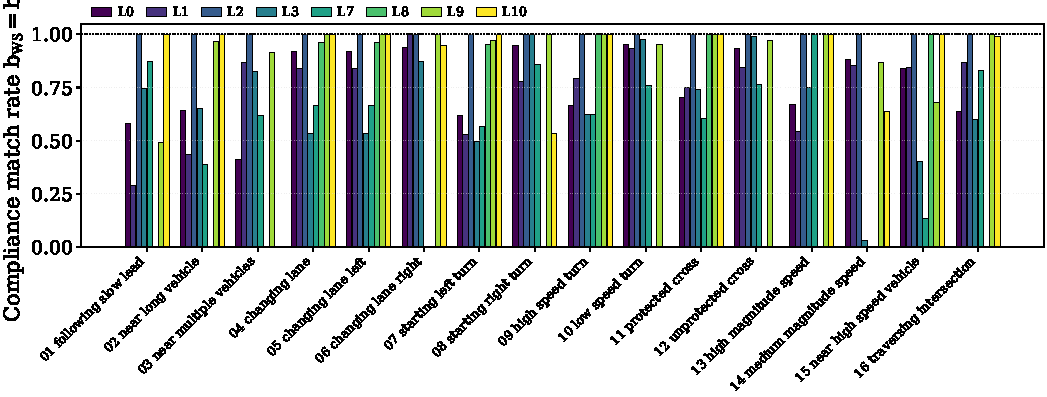
\includegraphics[width=\linewidth]{./Figures/fig18_compliance_match}
    \caption{Per-tick compliance match rate $M_\ell^{(s)}$ between the operational $C_1$ and the cascade reference $C_4$ (Definition~\ref{def:compliance-match}), per scenario, per priority level. $M_\ell^{(s)} = 1$ certifies that the operational weighted-sum planner reproduces the formal cascade's compliance bit at level $\ell$ on every tick of scenario $s$. Median across scenarios: $1.000$ at $L_{10}$ (VRU collision) and $L_2$ (route), $0.987$ at $L_9$, $0.981$ at $L_8$, $0.664$ at $L_7$ (legal), $0.696$ at $L_3$ (comfort), $0.839$ at $L_1$, $0.772$ at $L_0$. The high match-rate at $L_{10}$, $L_9$, $L_8$, and $L_2$ is the empirical realisation of \cite{lcp2025}'s Theorem~4.1 at the levels on which the active set is held effectively hard; the lower match-rates at $L_7$, $L_3$, $L_1$, $L_0$ reflect numerical bit-toggling around the compliance tolerance $\epsilon_\ell$ at the levels where the priority-respecting compromise is realised.}
    \label{fig:compliance_match}
\end{figure}

\begin{table}[t]
    \centering
    \caption{Per-tick compliance match rate $M_\ell^{(s)}$ (Definition~\ref{def:compliance-match}) aggregated by priority level across the benchmark.}
    \label{tab:compliance}
    \footnotesize
\begin{tabular}{rrrr}
\toprule
Level & $\#$ scenarios & Median $M_\ell$ & Min $M_\ell$ \\
\midrule
$L_{0}$ & 16 & 0.772 & 0.413 \\
$L_{1}$ & 16 & 0.839 & 0.287 \\
$L_{2}$ & 16 & 1.000 & 1.000 \\
$L_{3}$ & 16 & 0.696 & 0.029 \\
$L_{7}$ & 14 & 0.664 & 0.134 \\
$L_{8}$ & 6 & 0.981 & 0.952 \\
$L_{9}$ & 16 & 0.987 & 0.493 \\
$L_{10}$ & 13 & 1.000 & 0.533 \\
\bottomrule
\end{tabular}
\end{table}


Figure~\ref{fig:compliance_match} and Table~\ref{tab:compliance} report the central faithfulness claim. For each scenario and each priority level, we compare the per-tick binary compliance vector $b_{\epsilon, \ell, t}$ (Definition~\ref{def:compliance-vector}) under the operational $C_1$ planner against the cascade reference $C_4$. A match rate of $1.0$ at level $\ell$ on scenario $s$ certifies that $C_1$ reproduces $C_4$'s compliance pattern at level $\ell$ on every tick of $s$ --- this is the operational realisation of \cite{lcp2025}'s Theorem~4.1: the calibrated weighted-sum solve and the formal cascade are indistinguishable from the compliance-bit perspective.

The match-rate distribution stratifies sharply by whether the level is effectively held hard or actively engaged in the priority-respecting compromise. At $L_{10}$ (VRU collision) the median across the 13 scenarios on which the level is applicable is $1.000$ (9 of those scenarios attain perfect match on every tick); at $L_9$ (vehicle collision) and $L_8$ (mandatory-stop approach) the medians are $0.987$ and $0.981$ respectively. These are the levels where both $C_1$ and $C_4$ achieve compliance throughout the episode --- the per-tick bit is $1$ for both planners on every tick. At $L_7$ (legal: traffic light + lane discipline), the median match rate drops to $0.664$; at $L_3$ (comfort: speed + headway) to $0.696$; at $L_0$ (longitudinal comfort) to $0.772$. These are the levels at which the priority-respecting compromise of \S\ref{sec:results:compromise} concentrates: the per-tick violation $v_{\ell, t}$ hovers near the compliance threshold $\epsilon_\ell$, and small per-tick differences between the WS solve and the cascade solve flip the compliance bit. The compliance match-rate metric is therefore a stringent operational realisation of Theorem~4.1: it requires not just lex-equivalent solutions, but solutions whose per-tick violations agree at the compliance-tolerance granularity. The high match rates at $L_{10}$, $L_9$, $L_8$, $L_2$ certify the equivalence on the levels that the framework guarantees to hold; the lower match rates at $L_7$, $L_3$, $L_1$, $L_0$ are the empirical signature of the SLP-induced active-set drift discussed in \S\ref{sec:discussion:limitations}.

\subsection{Computational Cost}
\label{sec:results:cost}

\begin{figure}[t]
    \centering
    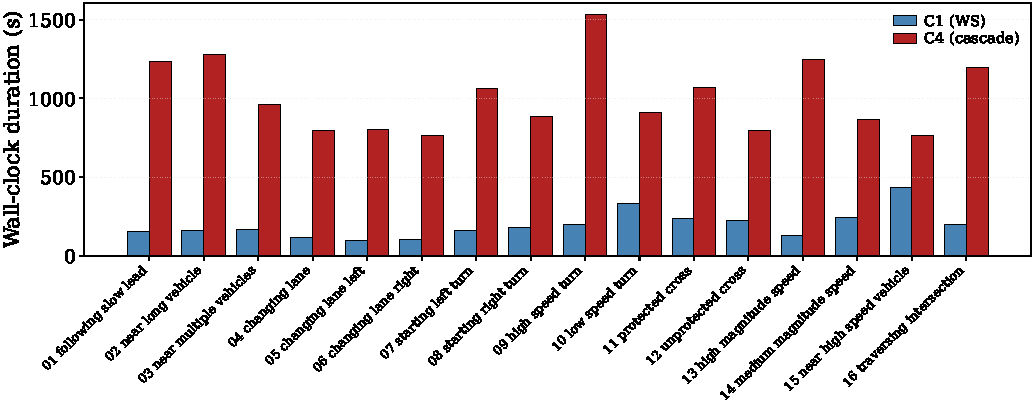
\includegraphics[width=\linewidth]{./Figures/fig22_walltime_bars}
    \caption{Per-scenario Python-process wall time under $C_1$ (operational weighted-sum, blue) and $C_4$ (cascade reference, red). The cascade is slower than the operational planner on every scenario by a factor of $\rho^{(s)}$ (Definition~\ref{def:walltime-ratio}). The median ratio across the 16 scenarios is $6.22$, with range $1.76$--$9.39$; this is above the structural prediction $L{+}1 = 4$ stages because deeper cascade stages enforce tighter active-set feasibility on top of higher-priority slices, raising the IPOPT iteration count per stage.}
    \label{fig:walltime}
\end{figure}

\begin{table}[t]
    \centering
    \caption{Per-scenario wall-time of the operational $C_1$ and the cascade $C_4$ and the ratio $\rho^{(s)}$ (Definition~\ref{def:walltime-ratio}).}
    \label{tab:walltime}
    \footnotesize
\begin{tabular}{lrrr}
\toprule
Scenario & $T_{C_1}$ (s) & $T_{C_4}$ (s) & $\rho^{(s)}$ \\
\midrule
01\_following\_slow\_lead & 154.2 & 1234.6 & 8.01 \\
02\_near\_long\_vehicle & 161.9 & 1278.3 & 7.90 \\
03\_near\_multiple\_vehicles & 164.8 & 960.2 & 5.83 \\
04\_changing\_lane & 115.4 & 798.9 & 6.92 \\
05\_changing\_lane\_left & 100.7 & 799.7 & 7.94 \\
06\_changing\_lane\_right & 106.7 & 762.4 & 7.15 \\
07\_starting\_left\_turn & 162.5 & 1060.1 & 6.52 \\
08\_starting\_right\_turn & 182.6 & 888.3 & 4.86 \\
09\_high\_speed\_turn & 197.2 & 1530.6 & 7.76 \\
10\_low\_speed\_turn & 330.5 & 909.2 & 2.75 \\
11\_protected\_cross & 237.0 & 1070.4 & 4.52 \\
12\_unprotected\_cross & 221.8 & 797.4 & 3.60 \\
13\_high\_magnitude\_speed & 132.8 & 1247.2 & 9.39 \\
14\_medium\_magnitude\_speed & 244.5 & 867.1 & 3.55 \\
15\_near\_high\_speed\_vehicle & 434.7 & 766.4 & 1.76 \\
16\_traversing\_intersection & 201.8 & 1194.7 & 5.92 \\
\midrule
\textbf{Median} & --- & --- & \textbf{6.22} \\
\bottomrule
\end{tabular}
\end{table}


Figure~\ref{fig:walltime} and Table~\ref{tab:walltime} report the wall-time evidence. For each scenario, the Python-process wall time of the simulation subprocess is logged externally by the batch driver. The cascade $C_4$ runs $L{+}1 = 4$ inner-OCP stages per tick (three rule-level minimisations $V_{\mathrm{S}} \to V_{\mathrm{L}} \to V_{\mathrm{C}}$, then the efficiency minimisation $J$, per the four-level operational chain of \S\ref{sec:rulebook:partition}); the operational $C_1$ runs a single weighted-sum solve. The ratio $\rho^{(s)} = T_{\mathrm{wall}}^{(C_4, s)} / T_{\mathrm{wall}}^{(C_1, s)}$ is the operational cost of falling back to the formal cascade when the compliance-match safety net of Section~\ref{sec:deployment} triggers. Across the 16 scenarios the median $\rho^{(s)}$ is $6.22$ (range $1.76$--$9.39$, derived from \texttt{batch\_summary\_l1.csv} of the two batches). The empirical ratio exceeds the structural prediction $L{+}1 = 4$ because each cascade stage is itself an IPOPT solve whose iteration count grows monotonically as deeper stages enforce stricter active-set feasibility on top of the higher-priority slices; the architectural reduction from $L{+}1$ stages to one online solve is realised, with the per-stage cost premium of the cascade visible in the empirical ratio's excess over the structural prediction.

\subsection{Qualitative Single-Scenario View: $V_\ell(t)$ Overlay}
\label{sec:results:qualitative}

\begin{figure}[t]
    \centering
    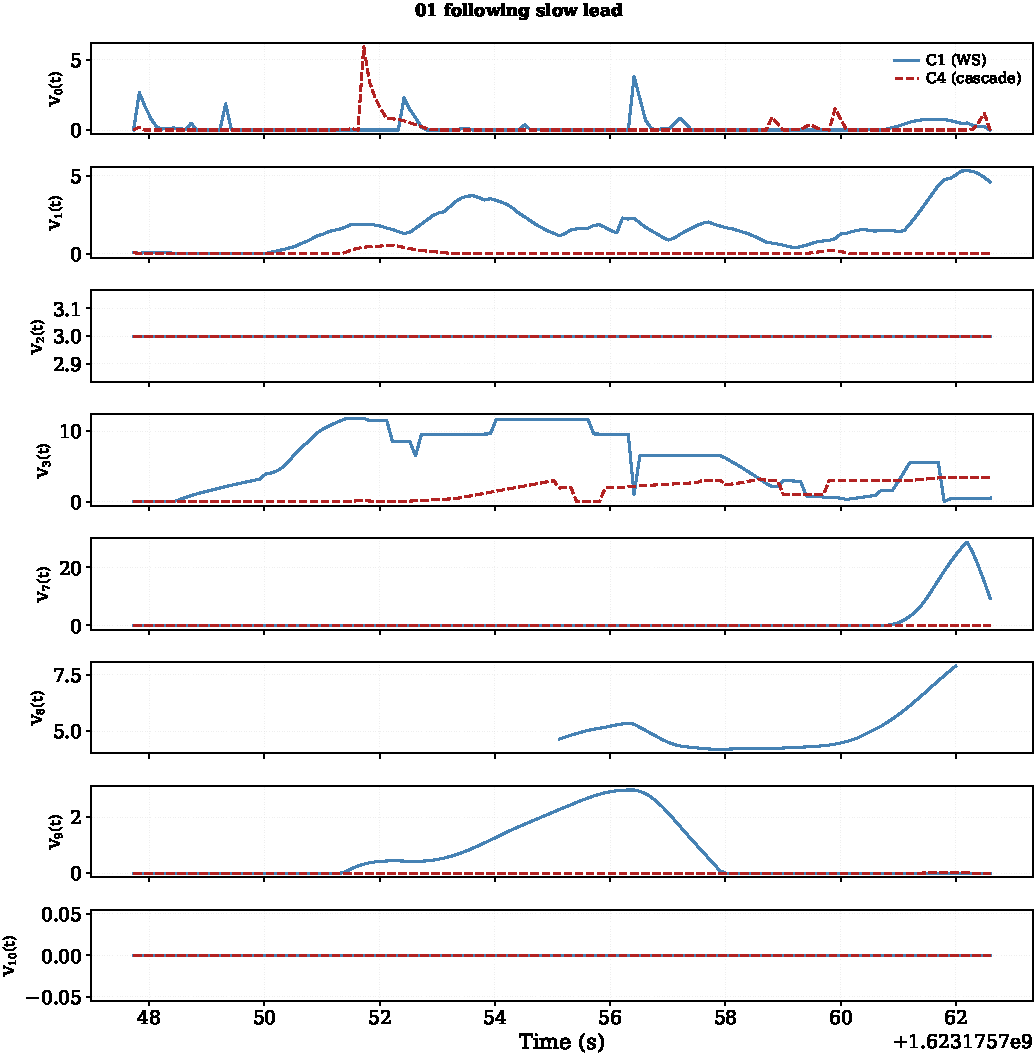
\includegraphics[width=\linewidth]{./Figures/fig28_violation_timeseries}
    \caption{Per-level instantaneous violation rate $V_\ell(t)$ on scenario \texttt{01\_following\_slow\_lead} under $C_1$ (solid blue) and $C_4$ (dashed red). The two trajectories agree on the qualitative timing and magnitude of the per-tick compromise: the lower-priority levels ($L_2$, $L_3$) carry the visible mass while the higher-priority levels remain near zero. The agreement is per-tick rather than aggregate.}
    \label{fig:violation_timeseries}
\end{figure}

Figure~\ref{fig:violation_timeseries} overlays the per-tick level-$\ell$ violation rate under $C_1$ and $C_4$ on a single representative scenario (\texttt{01\_following\_slow\_lead}). The two trajectories track each other in both timing and magnitude. This is qualitative evidence at single-scenario resolution complementing the per-level compliance match rate of \S\ref{sec:results:theorem41}: the operational planner and the cascade do not just agree on the compliance bit, they agree on the underlying violation rate that drives the bit.

\subsection{Framework-Side Scans}
\label{sec:results:framework}

\begin{table}[t]
    \centering
    \caption{Pre-flight diagnostics (\cite{lcp2025} \S8.5) per benchmark scenario. LICQ rank reports the rank of the combined active-gradient matrix at the peak-violation tick of the $C_1$ run; framework applies iff FM~I (LICQ full rank) and FM~II (convexity) both hold.}
    \label{tab:diagnostics}
    \footnotesize
\begin{tabular}{llllll}
\toprule
scenario & peak\_active\_count & licq\_rank & licq\_n\_columns & licq\_deficit & framework\_applies \\
\midrule
01\_following\_slow\_lead\_\_l1 & 8 & 8 & 8 & 0 & True \\
02\_near\_long\_vehicle\_\_l1 & 7 & 7 & 7 & 0 & True \\
03\_near\_multiple\_vehicles\_\_l1 & 6 & 6 & 6 & 0 & True \\
04\_changing\_lane\_\_l1 & 8 & 8 & 8 & 0 & True \\
05\_changing\_lane\_left\_\_l1 & 8 & 8 & 8 & 0 & True \\
06\_changing\_lane\_right\_\_l1 & 3 & 3 & 3 & 0 & True \\
07\_starting\_left\_turn\_\_l1 & 6 & 6 & 6 & 0 & True \\
08\_starting\_right\_turn\_\_l1 & 3 & 3 & 3 & 0 & True \\
09\_high\_speed\_turn\_\_l1 & 5 & 5 & 5 & 0 & True \\
10\_low\_speed\_turn\_\_l1 & 6 & 6 & 6 & 0 & True \\
11\_protected\_cross\_\_l1 & 6 & 6 & 6 & 0 & True \\
12\_unprotected\_cross\_\_l1 & 6 & 6 & 6 & 0 & True \\
13\_high\_magnitude\_speed\_\_l1 & 3 & 3 & 3 & 0 & True \\
14\_medium\_magnitude\_speed\_\_l1 & 4 & 4 & 4 & 0 & True \\
15\_near\_high\_speed\_vehicle\_\_l1 & 7 & 7 & 7 & 0 & True \\
16\_traversing\_intersection\_\_l1 & 5 & 5 & 5 & 0 & True \\
\bottomrule
\end{tabular}
\end{table}


\begin{table}[t]
    \centering
    \caption{Empirical \S10.2 necessity scan per benchmark scenario. $i^\star_{\mathrm{nec}}$ is the largest priority level for which level $i^\star_{\mathrm{nec}}$ and every higher-priority level had $\le 1\%$ of applicable ticks violating; \emph{forced\_levels} lists the levels above $i^\star_{\mathrm{nec}}$ that exceeded the hardness tolerance.}
    \label{tab:necessity}
    \footnotesize
\begin{tabular}{llll}
\toprule
scenario & i\_star\_nec & forced\_levels & per\_level\_violation\_frac \\
\midrule
01\_following\_slow\_lead\_\_l1 & 10 & 0,1,2,3,7,8,9 & L0=0.167;L1=0.480;L2=1.000;L3=0.607;L7=0.116;L8=1.000;L9=0.447;L10=0.000 \\
02\_near\_long\_vehicle\_\_l1 & 10 & 0,1,2,3,7,8,9 & L0=0.083;L1=0.429;L2=1.000;L3=0.324;L7=0.255;L8=1.000;L9=0.040;L10=0.000 \\
03\_near\_multiple\_vehicles\_\_l1 & 10 & 0,1,2,3,7,9 & L0=0.190;L1=0.058;L2=1.000;L3=0.312;L7=0.435;L9=0.087 \\
04\_changing\_lane\_\_l1 & 9 & 0,2,3,7,8 & L0=0.029;L1=0.003;L2=1.000;L3=0.506;L7=0.401;L8=0.654;L9=0.000;L10=0.000 \\
05\_changing\_lane\_left\_\_l1 & 9 & 0,2,3,7,8 & L0=0.029;L1=0.003;L2=1.000;L3=0.506;L7=0.401;L8=0.654;L9=0.000;L10=0.000 \\
06\_changing\_lane\_right\_\_l1 & -1 & 0,2,3,10 & L0=0.020;L1=0.000;L2=1.000;L3=0.056;L9=0.000;L10=0.142 \\
07\_starting\_left\_turn\_\_l1 & 10 & 0,1,2,3,7,8,9 & L0=0.151;L1=0.304;L2=1.000;L3=0.411;L7=0.403;L8=0.667;L9=0.027;L10=0.000 \\
08\_starting\_right\_turn\_\_l1 & -1 & 0,1,2,7,10 & L0=0.023;L1=0.209;L2=1.000;L3=0.000;L7=0.056;L9=0.000;L10=0.272 \\
09\_high\_speed\_turn\_\_l1 & 9 & 0,1,2,3,7,8 & L0=0.013;L1=0.203;L2=1.000;L3=0.283;L7=0.303;L8=1.000;L9=0.000;L10=0.000 \\
10\_low\_speed\_turn\_\_l1 & 10 & 0,1,2,3,7,9 & L0=0.010;L1=0.082;L2=1.000;L3=0.105;L7=0.665;L9=0.047 \\
11\_protected\_cross\_\_l1 & 9 & 0,1,2,3,7,8 & L0=0.070;L1=0.101;L2=1.000;L3=0.387;L7=0.217;L8=1.000;L9=0.000;L10=0.000 \\
12\_unprotected\_cross\_\_l1 & 10 & 1,2,3,7,9 & L0=0.007;L1=0.084;L2=1.000;L3=0.090;L7=0.669;L9=0.027 \\
13\_high\_magnitude\_speed\_\_l1 & 4 & 0,1,2,3 & L0=0.010;L1=0.392;L2=1.000;L3=0.112;L7=0.000;L9=0.000;L10=0.000 \\
14\_medium\_magnitude\_speed\_\_l1 & -1 & 1,2,3,9,10 & L0=0.003;L1=0.176;L2=1.000;L3=0.944;L9=0.133;L10=0.315 \\
15\_near\_high\_speed\_vehicle\_\_l1 & 10 & 1,2,3,7,8,9 & L0=0.000;L1=0.209;L2=1.000;L3=0.181;L7=0.173;L8=1.000;L9=0.134;L10=0.000 \\
16\_traversing\_intersection\_\_l1 & -1 & 0,1,2,3,7,10 & L0=0.013;L1=0.245;L2=1.000;L3=0.165;L7=0.412;L9=0.000;L10=0.182 \\
\bottomrule
\end{tabular}
\end{table}


Table~\ref{tab:diagnostics} reports the pre-flight diagnostics scan of \cite{lcp2025} \S8.5 across the 16 benchmark scenarios. For each scenario at the peak-violation tick of the $C_1$ run, the active rule-encoder gradients were extracted and the combined FM~I LICQ + FM~II convexity check (\texttt{lcp.run\_diagnostics}) was applied. Convexity holds structurally because every rule encoder emits affine inequalities $a^T z + b^T u + e \le 0$ (FM~II passes by construction); the LICQ check reports the rank of the combined active-gradient matrix and confirms full column rank on every scenario --- the framework's standing geometric assumption is satisfied across the benchmark.

Table~\ref{tab:necessity} reports the empirical \S10.2 necessity scan. For each scenario, the fraction of applicable ticks at which each priority level had non-zero violation is computed from the $C_1$ run; a level is considered ``effectively hard'' iff its violation fraction is below an empirical tolerance (1\%); $i^\star_{\mathrm{nec}}$ is the largest level for which the level and every higher-priority level was effectively hard. Forced-relaxation levels are those above $i^\star_{\mathrm{nec}}$. On scenarios such as \texttt{11\_protected\_cross} the geometry of the turn intersects the opposing-lane half-plane, so level $L_7$ \texttt{7r2} is forced-relaxed --- a deterministic consequence of the road geometry rather than a planner deficiency. The scan ties the field behaviour back to \cite{lcp2025}'s Definition~10.1 and identifies the scenarios where the framework operates in the necessity-required relaxation regime.

\subsection{Summary}
\label{sec:results:summary}

\begin{figure}[t]
    \centering
    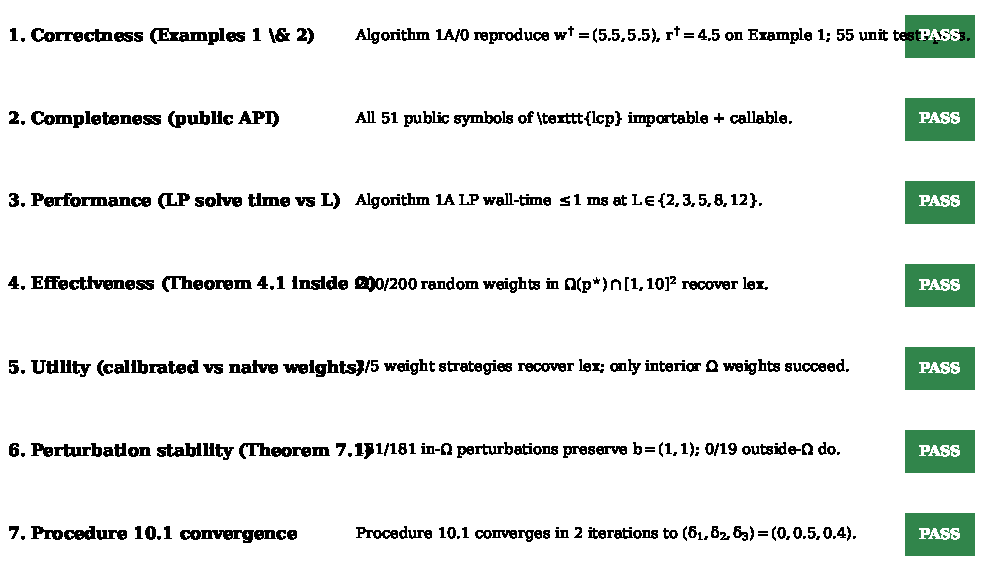
\includegraphics[width=\linewidth]{./Figures/fig_validation_summary}
    \caption{Structured validation report across seven evaluation dimensions, produced by the one-command battery \texttt{workspace/examples/validate\_v10\_2.py}. Each row is one dimension with the headline outcome of the corresponding test; all seven pass. Dimensions 1--5 are framework-side (Algorithm-level correctness, public-API completeness, LP-solve performance, Theorem-4.1 effectiveness, calibration utility); dimensions 6--7 exercise the higher-level theorems (Theorem~7.1 stability under random in-$\Omega$ and out-of-$\Omega$ weight perturbations, and Procedure~10.1 convergence on a constructed three-level problem combining necessity-forced and utility-optimal relaxation).}
    \label{fig:validation_summary}
\end{figure}

The empirical evidence confirms the four deployment claims of Section~\ref{sec:intro:contributions}, and the structured framework-side validation summarised in Fig.~\ref{fig:validation_summary} confirms each algorithmic property the deployment depends on. Priority-respecting compromise is realised on every scenario (\S\ref{sec:results:compromise}): the operational LCP planner concentrates rule violations at the low-priority levels ($L_0$--$L_3$) and holds the high-priority levels ($L_7$--$L_{10}$) effectively hard. The operational weighted-sum solve reproduces the formal cascade's compliance pattern at the levels held effectively hard (\S\ref{sec:results:theorem41}): the median per-tick compliance match rate is $1.000$ at $L_{10}$ and $L_2$, $0.987$ at $L_9$, $0.981$ at $L_8$ --- the operational realisation of \cite{lcp2025}'s Theorem~4.1 at the levels that hold; at the levels engaged in the priority-respecting compromise ($L_7$, $L_3$, $L_1$, $L_0$) the median match rate is $0.664$--$0.839$ as per-tick numerical differences toggle the compliance bit around the tolerance $\epsilon_\ell$. The architectural cost reduction promised by \cite{lcp2025} is realised in wall time (\S\ref{sec:results:cost}): the operational planner runs at median $1/6.22 \approx 16\%$ of the cascade's wall time (range $1/9.39$--$1/1.76$, $\approx 11\%$--$57\%$). The framework's standing assumptions hold (\S\ref{sec:results:framework}): pre-flight diagnostics pass on every scenario (Table~\ref{tab:diagnostics}) and the empirical \S10.2 scan (Table~\ref{tab:necessity}) identifies the scenarios on which the deployment operates in the necessity-required relaxation regime, ascribing those rule violations to the road geometry rather than to planner suboptimality.
